\chapter{Classification}
\label{classification}

\begin{comment}
	\section{Hardware resources}
	\label{hardwaree recources}
	\todo{vielleicht recources raus lassen}
	
	Multiple servers, provided by the cognitive system lab, were used. One of the provided servers is optimized for storing large amounts of data and was therefore used to store the histories and the results from the models during training while the other servers focus on computing power and were used to execute that training and evaluation. Mainly two servers were used for the training. One has the hardware specification shown in table \todo{ref} and the other one those shown in table \todo{ref}. 
	
	
	\begin{table}[H]
	\centering
	\caption{add caption}
	\label{mll-knecht}
	\resizebox{\columnwidth}{!}{%
	\begin{tabular}{l|ll}
	Component & Model & Additional details                   \\
	\hline
	Processing Unit    & Intel® Xeon® Gold Prozessor 5218      & 64 logical cores, \\
	&									& turbo boosts to 3,90 GHz \\
	System Memory      & -                      	           & 377 GB          \\
	Grafics            & 2 x NVIDIA RTX 2080 ti        		   & 11 GB graphics memory                   
	\end{tabular}
	}
	\end{table}
	
	\begin{table}[H]
	\centering
	\caption{add caption}
	\label{rechenknecht2}
	\resizebox{\columnwidth}{!}{%
	\begin{tabular}{l|ll}
	Component & Model & Additional details                   \\
	\hline
	Processing Unit    & Intel® Xeon® Prozessor E5-2650 v4     & 24 logical cores, \\
	&									& turbo boosts to 2,90 GHz \\
	System Memory      & -                      	           & 252 GB          \\
	Grafics            & NVIDIA GTX 1080 ti        		   & 11 GB graphics memory                   
	\end{tabular}
	}
	\end{table}
	
	\todo{specs nochmal checken sobald ich ins cartesium kann und da nachfragen. vor allem grafikkarte und hesteller des rams}
\end{comment}



\section{Models}
\label{models}
For determining whether subjects played a game without any obstacles or a game effected by the glare effect, one dimensional and two dimensional convolutional neural networks are utilized. As the task at hand is naturally a sequence classification, using 1D convnets is the more conventional approach of the two. 2D convnets on the other hand hand are almost universally used in computer vision applications \cite[Chapter~5]{cnn}. However, a possibility is to create synthetic images from the sequential data and use these images in a 2D convnet \cite{2dcnn}. The synthetic images are created in section \ref{2d_cnn_features} \nameref{2d_cnn_features}. The dimensions of the data and the feature maps in figure \ref{fig:1dCnnStructure} and \ref{fig:2dCnnStructure} are calculated for the case that all 20 rounds are used. If a different number of rounds is used the values differ. 

The models do not necessarily produce the best results possible since best practice 1D convnet \cite{1dcnn} and 2D convnet \cite{2dcnn} topologies are used. As the amount of collected real data with 20 recordings for each label is very limited, it was decided not to split the data into training, test and validation data, and instead only into training and test data using leave-one-out cross validation, where each model is trained with data from n-1 subjects and thus tested on the data from the remaining subject \cite[Chapter~1]{oneOut}. As there is no separate validation set, an optimization would have to be done on the test data. If the parameters are optimized using the test set, the measurement of generalization would be flawed \cite[Chaper~4]{cnn}. Therefore, it was avoided to optimize the hyper parameters individually for each model to ensure generalizing on new testing data. Instead, common best practice hyper parameters were optimized over all the models for better generalizing ability.

%In order to optimize the models a separate validation set would be neccessary. It could be used to tune the hyper parameters of the model and the models would be tested on the test data that was not part of the process of the optimization. 

%The reason why the optimization is done on a separate validation set is, that the models can then be tested on the test data which was not part of the process of selecting the best hyper parameters. If the models were optimized using the test data, the results would not be representitive of the performance of the models on unknown data. 

%The cnn models are intentionally created not very complex for two reasons: Firstly, a lot of training needs to be done with differnet configurations regarding the steps included and the ratios of simulkated to real data. As mentioned in \todo{ref}, 76800 models need to be trained. As the time this work is created in is limited, training that many complex models would take too long. Especially the training of the 2d cnns requires a lot of time. Secondly, to assure that the structures are complex enough, more complex models were exemplary trained and they showed either similar or worse performance. The results of the more complex models can be see in the appendix \todo{ref?}. 

%only difference is input size depending on the number of round included. 

%\todo{statt begründung die quellenangeben. Von wo..}


\begin{comment}
	The visualisations are based (and heavily adjusted) on the latex code provided by the following license:
	
	MIT License
	
	Copyright (c) 2018 HarisIqbal88
	
	Permission is hereby granted, free of charge, to any person obtaining a copy
	of this software and associated documentation files (the "Software"), to deal
	in the Software without restriction, including without limitation the rights
	to use, copy, modify, merge, publish, distribute, sublicense, and/or sell
	copies of the Software, and to permit persons to whom the Software is
	furnished to do so, subject to the following conditions:
	
	The above copyright notice and this permission notice shall be included in all
	copies or substantial portions of the Software.
	
	THE SOFTWARE IS PROVIDED "AS IS", WITHOUT WARRANTY OF ANY KIND, EXPRESS OR
	IMPLIED, INCLUDING BUT NOT LIMITED TO THE WARRANTIES OF MERCHANTABILITY,
	FITNESS FOR A PARTICULAR PURPOSE AND NONINFRINGEMENT. IN NO EVENT SHALL THE
	AUTHORS OR COPYRIGHT HOLDERS BE LIABLE FOR ANY CLAIM, DAMAGES OR OTHER
	LIABILITY, WHETHER IN AN ACTION OF CONTRACT, TORT OR OTHERWISE, ARISING FROM,
	OUT OF OR IN CONNECTION WITH THE SOFTWARE OR THE USE OR OTHER DEALINGS IN THE
	SOFTWARE.
\end{comment}

\newpage

\subsection{1D convnet}
\label{1d_cnn}
The structure of the 1D convnet used is shown in figure \ref{fig:1dCnnStructure}.
\begin{figure}[H]
	\centering
	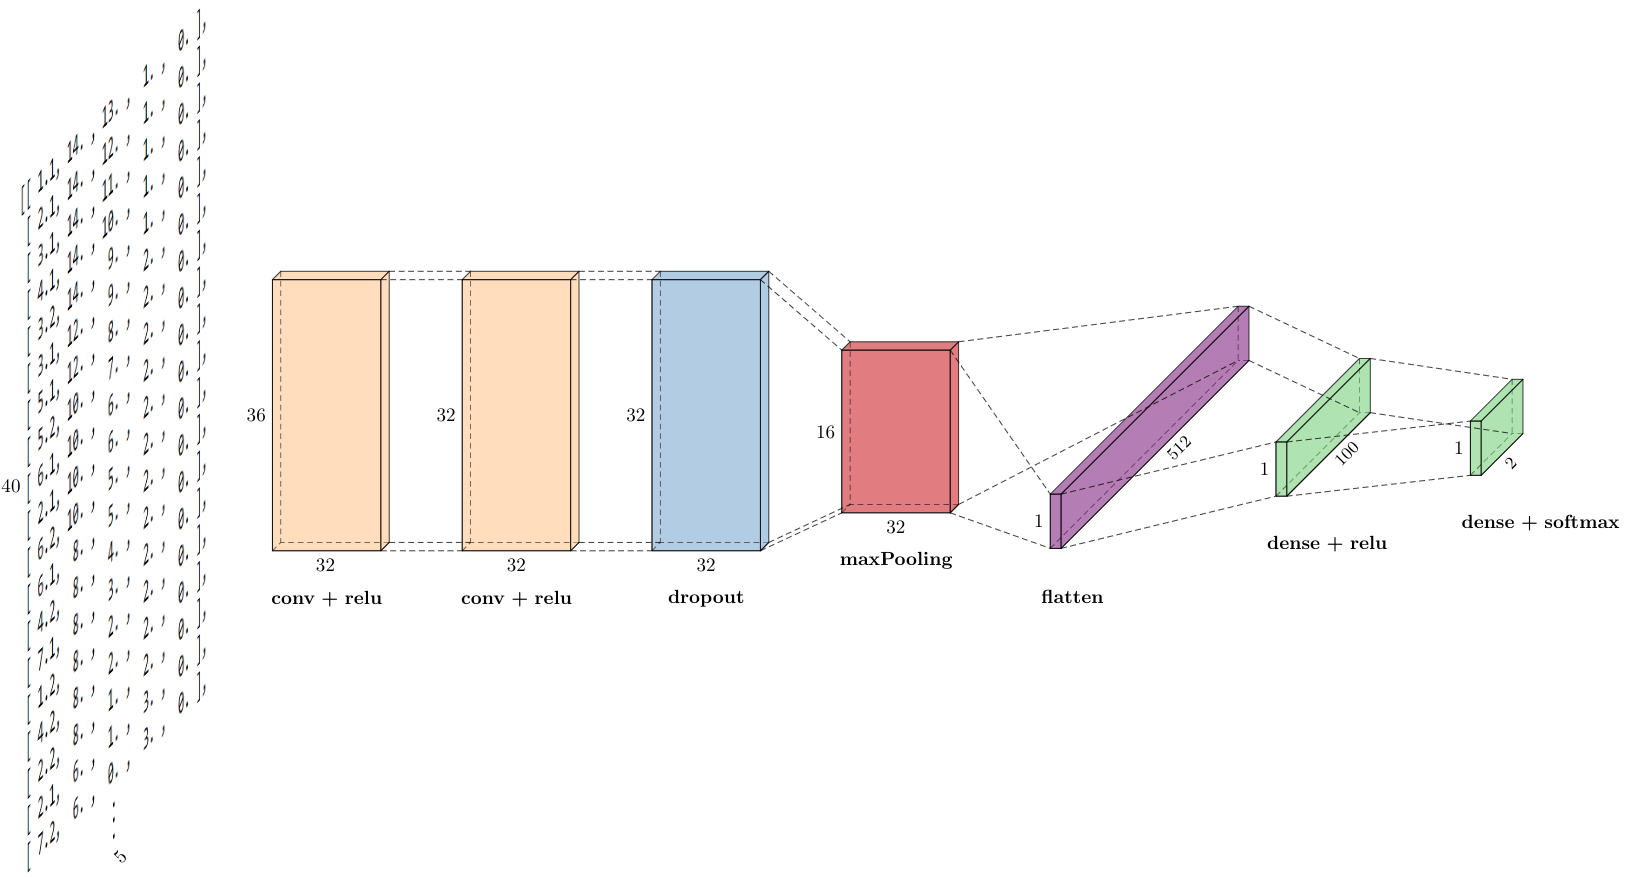
\includegraphics[width=15cm]{images/1dCnnStructureChanged.png}
	\caption[Visualization of the utilized 1D convnet topology.]{Visualization of the utilized 1D convnet topology. The dimensions represent those of the feature map in that layer. For example, the first convolution layer produces a feature map with the size 36 x 32 with 32 being the number of filters computed.\\ The input is on the left and the output on the right.}
	\label{fig:1dCnnStructure}
\end{figure}
The input data consist of the 5 statistical features, explained in section \ref{1d_cnn_features} \nameref{1d_cnn_features}, for each of the 40 steps (20 rounds), resulting in the input dimensions 40 x 5. Initially the data is passed to the first convolution layer of the network. The first layer computes 32 filters and the convolutional kernel has a size of 5, meaning that every step from the kernel includes all data from 5 steps in the game. The resulting feature map has a size of 36 x 32. This feature map is passed to the second convolution layer that computes the same number of filters. The kernel also has the same size like in the first layer. This results in a feature map with a size of 32 x 32. Afterwards, a dropout layer with a rate of 0.5 randomly sets input features to 0 to reduce overfitting. Then a one dimensional max-pooling layer with a pool size of 2 reduces the size of the feature map to 16 x 32. Afterwards, a flatten layer forms the features into one dimension. These features are finally passed to a densely connected network, consisting of two dense layers. Both convolution layers, and the first dense layer use a rectified linear unit as activation function. The last dense layer uses softmax as activation function to bring the data down to two values that specify the result of the classification. In total 57486 parameters are trained in this model. 

For the optimization, the Adam algorithm is used that is already implemented in Keras. Adam optimization is a stochastic gradient descent method \cite{keras}. The learning rate is set to 0.0001 and not changed during the training. The batch size is set to 32 and the model is trained for 2500 epochs. 
%Later many models had to be retrained due to complications and the epochs were reduced to 1500, because 2500 was unnecessarily high (accuracy continually decreased already after less than 1500 epochs).% As mentioned before, this is a best practice configuration

%As mentioned before, this is a best practice configuration, optimized over all the 1D convnet models and not individually for each model. 

\newpage

\subsection{2D convnet}
\label{2d_cnn}
The structure of the 2D convnet used is shown in figure \ref{fig:2dCnnStructure}.
\begin{figure}[H]
	\centering
	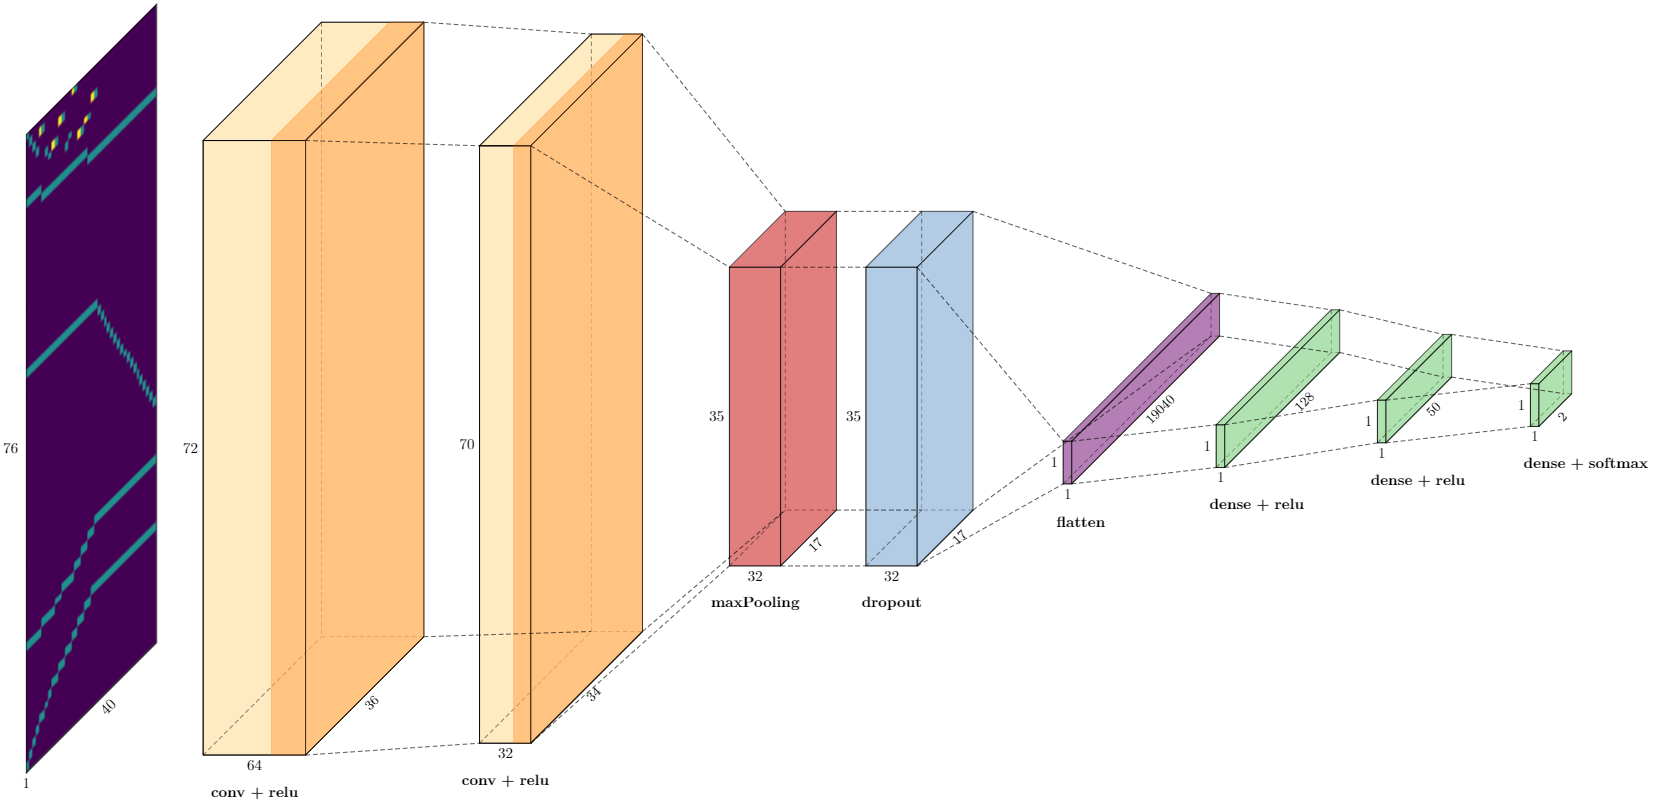
\includegraphics[width=15cm]{images/2dCnnStructure_new.png}
	\caption[Visualization of the utilized 2D convnet topology.]{Visualization of the utilized 2D convnet topology. The dimensions represent those of the feature map in that layer. For example, the first convolution layer produces a feature map with the size 72 x 36 x 64 with 64 describing the number of filters computed.\\ The input is on the left and the output on the right.}
	\label{fig:2dCnnStructure}
\end{figure}
The input data consist of the synthetic images generated in section \ref{2d_cnn_features} \nameref{2d_cnn_features}, using the 5 statistical features. This results in the input dimensions 76 x 40 x 1. Initially the data is passed to the first convolution layer of the network. It computes 64 filters and the convolutional kernel has a size of 5 x 5, meaning that each step from the kernel includes a 5 x 5 sized area of the synthetic image. This convolution results in a feature map with a size of 72 x 36 x 64. This feature map is passed to the second convolution layer that computes 32 filters with a kernel of size of 3 x 3. This results in a feature map with the size of 70 x 34 x 32. Then a two dimensional max pooling layer with a pool size of 2 x 2 reduces the size of the feature map to 35 x 17 x 32. Afterwards, a dropout layer with a rate of 0.2 randomly sets input units to 0 to reduce overfitting. Then a flatten layer forms the features into one dimension. These features are finally passed to a densely connected network, consisting of three dense layers. Both convolution layers, and the first two dense layers use a rectified linear unit as activation function. The last dense layer uses a softmax activation function to bring the data down to two values that specify the result of the classification. In total 2463928 parameters are trained in this model.

For the optimization, the Adam algorithm is used that is already implemented in Keras. Adam optimization is a stochastic gradient descent method \cite{keras}. The learning rate is set to 0.00001 and not changed during the training. The batch size is set to 32 and the model was initially trained for 500 epochs. Later, many 2D convnets had to be retrained due to complications and the epochs were reduced to 200, because 500 was unnecessarily high (accuracy continually decreased already after less than 500 epochs). This can be seen in figure \ref{fig:2d40}. 
% As mentioned before, this is a best practice configuration. 

%As mentioned before, this is a best practice configuration, optimized over all the 2D convnet models and not individually for each model. 

\begin{comment}

\subsubsection{Visualizing intermediate activations}
\todo{vielleichtz diese section rausnehemen. ich denke es ist unnötig, weil es nicht dazu beiträgt was meine arbeit zeigen soll}

An interesting thing about 2d cnns is that it is possible to vizualize the reprenestations learned by the network. This helps to understand the meaning of individual filters. Intermediate activations canm be vizualized by displaying the feauture maps that are the outpu of various convolution and pooling layers in the network, given an image is passed to the input layer. \todo{ref} To extract these feature maps, the model is first trained for one split and then run in prediction mode. Vizualizing each feature map produced by filters gives a view into how an input is decomposed into the different filters learned by the cnn. The decision was made not to focus too much on vizualizing all feature maps but instead to only vizualize one feature map created by each layer. As each feature map can learn different features, the following visualizations are only small fractions of what the cnn learns. Thgerefore they should only serve as exemplary illustration of what the different layers of the cnn output.

\todo{bisschen beschreiebn was was ist von den bildern und was man sieht}

\begin{minipage}{0.5\textwidth}
\begin{figure}[H]
\centering
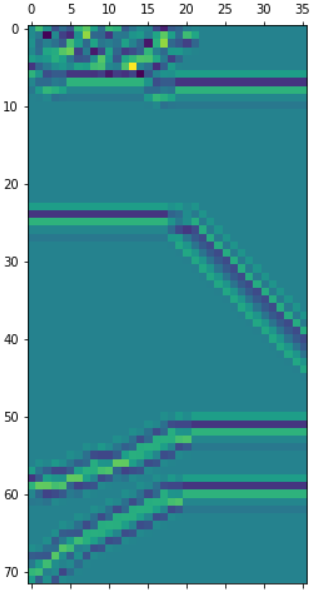
\includegraphics[width=5cm]{images/2dcnnLayer1.png}
\caption[Bild kurz]{Add caption}
\label{fig:vis2d1}
\end{figure}
\end{minipage}
\begin{minipage}{0.5\textwidth}
\begin{figure}[H]
\centering
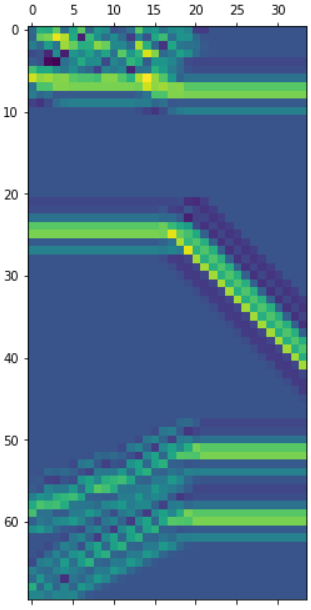
\includegraphics[width=5cm]{images/2dcnnLayer2.png}
\caption[Bild kurz]{Add caption}
\label{fig:vis2d2}
\end{figure}
\end{minipage}

\begin{minipage}{0.5\textwidth}
\begin{figure}[H]
\centering
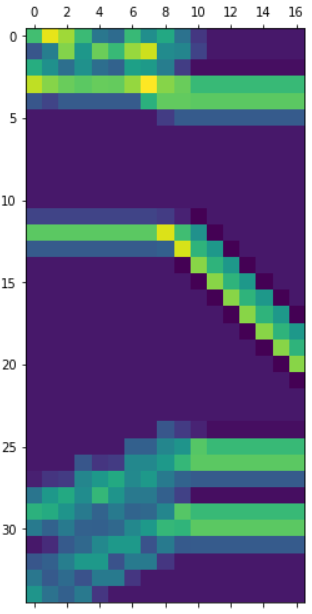
\includegraphics[width=5cm]{images/2dcnnLayer3.png}
\caption[Bild kurz]{Add caption}
\label{fig:vis2d3}
\end{figure}
\end{minipage}
\begin{minipage}{0.5\textwidth}
\begin{figure}[H]
\centering
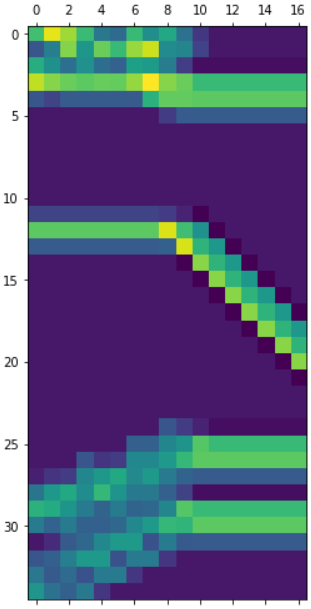
\includegraphics[width=5cm]{images/2dcnnLayer4.png}
\caption[Bild kurz]{Add caption}
\label{fig:vis2d4}
\end{figure}
\end{minipage}

It can be seen that the original structure of the image is still recognizable after all convolutional, pooling and dropout layers. When dealing with cnns that have more layers, usually the original image is at some point not recognizable anymore. The remaining layers of the 2d cnn effectively opperate on one dimensionaml data and create the output. Therfore they will be left out in this vizualization.


%Especially when dealing with more copmplex structures of cnns, vizualizing all feature maps instead of one, can reveal valuable informations. Generelly, the deeper the layer, the less of the original image is recogniazable. Since the size of the 2d cnn used is comparetively small, the original image is still recognizable after all convolutional, poolind and dropout layers.  For instance can be analysed if the structure of the cnn is overly complex for the data. This is the case if the last layers do not activate anymore, as there is nothing more to learn at that point, resulting in all values of the feature maps being 0. 


%If this technique is used for actually analysisng the cnn,  



%An interesting thing about 2d cnns, what is not possible to that extend in most of the neural networks, is that the steps in between can be vizualized. As each convolutional layer creates new images using the filters, it is actually possible to look at the images between layers. Generelly the deeper the layer the less from the actual image is recognizable. It can be observed how the network step by step forms the input image to the output shape. Although this is not especially usefull for actually knowing what the network does, it is usefull for knowing if certain layers of the network do something at all. If for instance the structure of the cnn is overly complex for the data, this will be indicated by the fact that the last layers are not activating at all becuase there is nothing more to learn at that point (all values of all feature maps from a layer are 0). Although the structure of the 2d cnn used is not very complex and this technique is more relevant for larger networks, it is interesting to exemplary look at the images between the convolutions of the 2d cnn used. To do so the model is first trained for one split and then run in predict mode. When passing an image to the imput layer it is then possible to extract the images between layers.

\todo{da wird ein buch erwähnt, wo der typ erzählt wieso es gut ist das zu machen. Die zitate umschreiben in meinen text: \url{https://towardsdatascience.com/visualizing-intermediate-activation-in-convolutional-neural-networks-with-keras-260b36d60d0}}

%... bild..

%As visible, there are no layers from which all filters do not activate, meaning the structure is not overly complex for the data. 

%\todo{referenz finden und bilder einbinden von dem 2d cnn. vielleicht auch ein bild von einem größeren netz wo es nichts mehr lernt.}

\end{comment}

\newpage

\section{Training setup}
\label{training_setup}
There is one script each for training the 1D convnet and the 2D convnet. The only differences are in the structure and the hyper parameters of the convnets and that before training the 2D convnet the loaded statistical features must first be used to create the synthetic images. Both scripts load the same statistical features, already divided into 20 splits that are used for leave-one-out cross validation. Each split contains a training and a test set. A training set consists of 19 real and 19000 simulated games for each of the two classes, while a test set contains one real game for each of the classes. The 2000 simulated games excluded from the training are not used for testing, because the results would not be representative of the real world performance of the models. Furthermore, only a certain number of the best simulations are included in the training. The ratio of n simulated games for each real games will be abbreviated with sdnx. For instance, sd5x means that 5 simulated games for each real game were included in the training. 
%As there are statistical features for 20 real and 20000 simulated no obstacles games as well as the same amount for glare effects games, this results in each split containing data from 19 real and 19000 simulated games for each of the two classes, resulting in 38 real and 38000 simulated games available for the training. From 2 real and 2000 simulated games not used for training, only the data from the real games is used for testing. \todo{leave one out cross validation erwähnen, generell umformulieren weil es maximal so viele simulierte sind und nicht generell} Testing on simulated data would not be representative of the real world performance of the models. Furthermore it can be chosen for which ratios between simulated and real games models should be trained. 
Each training of a model is done for the following ratios: sd0x, sd1x, sd2x, sd3x, sd4x, sd5x, sd6x, sd7x, sd8x, sd9x, sd10x and sd20x. Moreover, the training is done on different numbers of rounds (each round consists of flipping two cards). In real world scenarios, the less turns waited the faster the decision is made and assistance can be applied. However, if waited longer the decision will likely be correct more often. To analyse this, the models are trained each for 5, 10, 15 and 20 rounds. More than 20 turns were not recorded. As convnets are stochastic machine learning algorithms, different runs of the same algorithm on the same data can result in different outcomes. Therefore, it is not sufficient to train each model only once as the result is not reliable. Instead, the training of a model is repeated multiple times and the results are averaged to summarize the performance of the model \cite{repetition}. The decision was made to repeat the training of each model 20 times. 
% Training models for ranges of turns in the middle, for instance from turn 10 to 15, was left out, because this is not very interesting when conscidering real world usage. 

%All models are trained twice. Once on the simulated data created before modifying the simulator and once afterwards. This can potentially show whether the changes improved the classification results. 

%As mentioned in chapter \todo{ref}, the topology

%The structure and hyper parameters of the modells for all 1d cnns are identical. Same goes for all 2d models. The only differnece is the input shape of the modells since it depends on teh number of steps used in the training. Identical structure for modells of the same type are used so that different training results for different amount of steps can be reliably compared. It should be noted the structure and hyper paramters are not the same between the 1d and 2d cnns. 

Once one of the scripts is executed, required directory structures are created and training processes for the different ratios of real to simulated games are performed successively. The training for one ratio consists of parallelized training of 20 splits using multiprocessing. As the training for each split is repeated 20 times, for each ratio 20 models are created  for every split. This means that 400 models are trained for every ratio. As there are 12 different ratios trained, this results in 4800 models trained for each execution of one of the scripts. As mentioned above, the training is done for 4 different amounts of rounds for the 1D convnet and the 2D convnet. This adds up to 38400 models being trained. Furthermore, this is done twice: Once before the changes to the simulator and once afterwards, to see if the changes improved the performance of the models. All in all, this results in 76800 models. For each model the training history is saved in a file. Saving and loading the histories is necessary due to the parallel training of multiple models through multiprocessing. Once the training of the 4800 models of one script is completed, the training histories are loaded from the files. The results from the 400 training histories for each ratio of real to simulated games are averaged, plotted and the final figures are saved for the analysis.
% The reason for averaging the results over many models is, that deep neural networks by default initialize their weights randomly, resulting in potentially different outcomes of each training \todo{stattdessen begründung mit stochastic models mit referenz}. By averaging the results, the values and therefore the interpretation becomes more reliable and meaningful. 
All models are trained on the CPU. The fact that 76800 models are trained led to the decision, not to save all models but instead first evaluate the results and then retrain and save the models that create the best results thus using less memory.  

\begin{comment}


There are two main folders for storing the classification results. One for the results before the changes to the simulator and the other one for the results afterwards. Once one of the training scripts is executed, a subfolder for saving and loading 
The scripts create and use a specific directory structure conceptualized in figure \todo{ref}.
structure erklären

resutls -> 2d... -> sdxordner,(sdx images) -> split1 -> run1resutls 

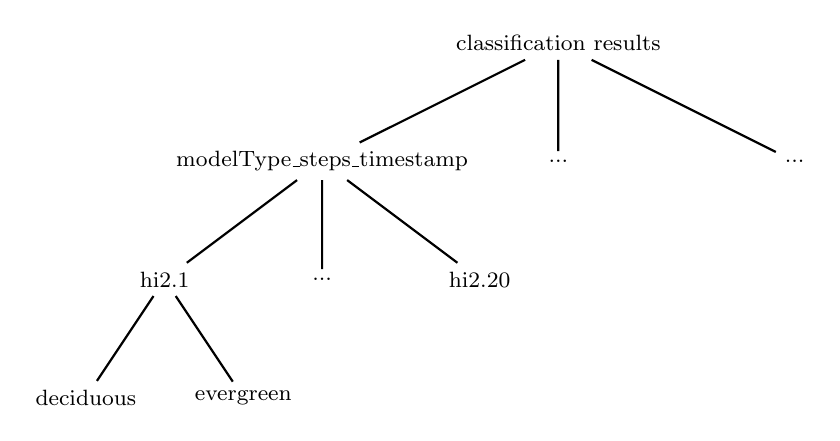
\begin{tikzpicture}
[sibling distance=3cm,-,thick]
\footnotesize
\node {classification results}
child {node {modelType\_steps\_timestamp}
	[sibling distance=2cm]
	child {node {hi2.1}
		child {node {deciduous}}
		child {node {evergreen}}
	}
	child {node {...}}
	child {node {hi2.20}}
}
child {node {...}
}
child {node {...}
}
;
\end{tikzpicture}

\end{comment}

\newpage
   
\section{Training results and evaluation}
\label{training_results_and_evaluation}
The training results for the various configurations can be seen in table \ref{tab:1d_before}, \ref{tab:2d_before}, \ref{tab:1d_after} and \ref{tab:2d_after}. The first two tables contain the results before the changes to the simulator and the last two the results afterwards. The analysis will only focus on the accuracy, but the loss is also listed for the sake of completeness. The best accuracies for each number of turns in each table are highlighted in green. If multiple ratios of real to simulated games for a certain number of turns produce the same accuracy only the one with the smallest amount of simulations is highlighted. The accuracies in the tables are those from the best epochs. In most of the cases the models start overfitting after a certain epoch resulting in a deterioration of the accuracy after reaching a local maximum. In rare cases the test accuracy converges. Such a case can be observed in figure \ref{fig:1d20}.
%All models except the 1D convnet for 5 rounds and ratios of sd0x and sd1x reach such a local maximum in accuracy before the training is stopped. 

It should be clarified that the chosen configurations of models to be trained make no claim to completeness and do not claim to produce the best results, as they are not optimized individually. In all following tables the word round is abbreviated with r. and accuracy with acc. 


\newpage

\begin{comment}
	\begin{table}[H]
	\centering
	
	\resizebox{0.9\columnwidth}{!}{%
	\begin{tabular}{|c||ccccc|ccccc|ccccc|ccccc|}
	\hline
	&&& 5 r. &&&&& 10 r. &&&&& 15 r. &&&&& 20 r. &&\\
	\hline
	&& Acc. && Loss &&& Acc. && Loss &&& Acc. && Loss &&& Acc. && Loss &\\
	\hline\hline
	sd0x &&     65.12\% && 0.6584 &&& \textbf{\textcolor{mygreen}{81.12\%}} && 0.5116 &&& \textbf{\textcolor{mygreen}{78.37\%}} && 0.5377 &&& 79.62\% && 0.492 &\\
	sd1x &&     71.25\% && 0.6385 &&& 80.88\% && 0.4777 &&& 77.25\% && 0.5355 &&& 80.12\% && 0.4999 &\\
	sd2x &&     68.5\% && 0.6476 &&& 77.38\% && 0.5283 &&& 78.25\% && 0.5275 &&& \textbf{\textcolor{mygreen}{81.25\%}} && 0.4887 &\\
	sd3x &&     69.38\% && 0.6494 &&& 75.5\% && 0.5252 &&& 76.13\% && 0.5329 &&& 79.75\% && 0.4999 &\\
	sd4x &&     67.5\% && 0.6436 &&& 75.88\% && 0.538 &&& 77.25\% && 0.5322 &&& 81.25\% && 0.4975 &\\
	sd5x &&     72.25\% && 0.6212 &&& 76.5\% && 0.5252 &&& 77.75\% && 0.5338 &&& 81.25\% && 0.4985 &\\
	sd6x &&     71.87\% && 0.6346 &&& 74.75\% && 0.547 &&& 76.25\% && 0.5376 &&& 79.38\% && 0.5075 &\\
	sd7x &&     70.25\% && 0.6252 &&& 73.62\% && 0.5395 &&& 76.0\% && 0.5326 &&& 80.0\% && 0.5078 &\\
	sd8x &&     74.25\% && 0.6121 &&& 72.5\% && 0.5509 &&& 77.0\% && 0.535 &&& 79.75\% && 0.4993 &\\
	sd9x &&     \textbf{\textcolor{mygreen}{74.88\%}} && 0.5826 &&& 74.63\% && 0.5483 &&& 76.0\% && 0.542 &&& 81.75\% && 0.4987 &\\
	sd10x &&    74.87\% && 0.5971 &&& 74.5\% && 0.5558 &&& 77.12\% && 0.5394 &&& 80.87\% && 0.5036 &\\
	sd20x &&    73.25\% && 0.5831 &&& 73.5\% && 0.5493 &&& 75.63\% && 0.5355 &&& 80.75\% && 0.5013 &\\
	\hline
	\end{tabular}
	}
	\caption[Best accuracies and losses produced by the 1D convnet. Before the changes to the simulator.]{Best accuracies and losses for 5, 10, 15 and 20 rounds produced by the 1D convnet. Before the changes to the simulator.}
	\label{tab:1d_before_old}
	\end{table}
\end{comment}

\begin{table}[H]
	\centering
	
	\resizebox{0.9\columnwidth}{!}{%
		\begin{tabular}{|c||ccccc|ccccc|ccccc|ccccc|}
			\hline
			&&& 5 r. &&&&& 10 r. &&&&& 15 r. &&&&& 20 r. &&\\
			\hline
			&& Acc. && Loss &&& Acc. && Loss &&& Acc. && Loss &&& Acc. && Loss &\\
			\hline\hline
			sd0x &&     65.12\% && 0.6584 &&& \textbf{\textcolor{mygreen}{81.88\%}} && 0.507 &&& \textbf{\textcolor{mygreen}{78.63\%}} && 0.5415 &&& 78.75\% && 0.5039 &\\
			sd1x &&     71.25\% && 0.6385 &&& 81.75\% && 0.4899 &&& 77.38\% && 0.5399 &&& 80.62\% && 0.4893 &\\
			sd2x &&     68.5\% && 0.6476 &&& 77.38\% && 0.5128 &&& 77.25\% && 0.539 &&& 80.0\% && 0.4965 &\\
			sd3x &&     69.38\% && 0.6494 &&& 77.5\% && 0.5135 &&& 75.75\% && 0.5364 &&& 79.88\% && 0.4928 &\\
			sd4x &&     67.5\% && 0.6436 &&& 77.5\% && 0.5446 &&& 76.13\% && 0.5418 &&& \textbf{\textcolor{mygreen}{81.12\%}} && 0.501 &\\
			sd5x &&     72.25\% && 0.6212 &&& 74.5\% && 0.5404 &&& 78.25\% && 0.5286 &&& 81.0\% && 0.5005 &\\
			sd6x &&     71.87\% && 0.6346 &&& 75.25\% && 0.5412 &&& 77.12\% && 0.5356 &&& 80.25\% && 0.4967 &\\
			sd7x &&     70.25\% && 0.6252 &&& 73.38\% && 0.5453 &&& 75.63\% && 0.5357 &&& 81.12\% && 0.4918 &\\
			sd8x &&     74.25\% && 0.6121 &&& 73.38\% && 0.5486 &&& 77.0\% && 0.5316 &&& 80.38\% && 0.5036 &\\
			sd9x &&     \textbf{\textcolor{mygreen}{74.88\%}} && 0.5826 &&& 74.25\% && 0.5369 &&& 76.5\% && 0.5408 &&& 80.25\% && 0.4909 &\\
			sd10x &&    74.87\% && 0.5971 &&& 76.38\% && 0.5594 &&& 76.25\% && 0.548 &&& 80.25\% && 0.501 &\\
			sd20x &&    73.25\% && 0.5831 &&& 73.25\% && 0.5414 &&& 76.0\% && 0.5387 &&& 80.87\% && 0.4935 &\\
			\hline
		\end{tabular}
	}
	\caption[Best accuracies and losses produced by the 1D convnet, prior to the changes to the simulator.]{Best accuracies and losses for 5, 10, 15 and 20 rounds produced by the 1D convnet, prior to the changes to the simulator.}
	\label{tab:1d_before}
\end{table}

\begin{table}[H]
	\centering
	
	\resizebox{0.9\columnwidth}{!}{%
	\begin{tabular}{|c||ccccc|ccccc|ccccc|ccccc|}
		\hline
		&&& 5 r. &&&&& 10 r. &&&&& 15 r. &&&&& 20 r. &&\\
		\hline
		&& Acc. && Loss &&& Acc. && Loss &&& Acc. && Loss &&& Acc. && Loss &\\
		\hline\hline
		sd0x &&     63.5\% && 0.6471 &&& 74.0\% && 0.4991 &&& 79.62\% && 0.4726 &&& 79.0\% && 0.4778 &\\
		sd1x &&     68.12\% && 0.619 &&& 76.62\% && 0.5171 &&& 79.5\% && 0.4984 &&& 81.75\% && 0.4735 &\\
		sd2x &&     68.25\% && 0.6382 &&& \textbf{\textcolor{mygreen}{80.0\%}} && 0.5243 &&& 80.38\% && 0.4851 &&& 84.12\% && 0.4573 &\\
		sd3x &&     69.5\% && 0.6392 &&& 78.88\% && 0.5518 &&& 80.25\% && 0.5038 &&& 84.62\% && 0.4718 &\\
		sd4x &&     67.63\% && 0.6415 &&& 76.38\% && 0.5685 &&& 79.62\% && 0.5106 &&& \textbf{\textcolor{mygreen}{85.0\%}} && 0.4726 &\\
		sd5x &&     70.88\% && 0.6339 &&& 74.63\% && 0.5668 &&& 80.0\% && 0.51 &&& 84.88\% && 0.474 &\\
		sd6x &&     70.62\% && 0.638 &&& 77.0\% && 0.5623 &&& 80.12\% && 0.5077 &&& 84.88\% && 0.4776 &\\
		sd7x &&     69.75\% && 0.6543 &&& 75.38\% && 0.5762 &&& 79.5\% && 0.5176 &&& 85.0\% && 0.4839 &\\
		sd8x &&     70.0\% && 0.6467 &&& 74.25\% && 0.5775 &&& 80.38\% && 0.5164 &&& 85.0\% && 0.484 &\\
		sd9x &&     71.25\% && 0.6395 &&& 78.75\% && 0.5696 &&& \textbf{\textcolor{mygreen}{81.5\%}} && 0.5064 &&& 85.0\% && 0.4814 &\\
		sd10x &&    68.75\% && 0.6296 &&& 77.75\% && 0.5674 &&& 80.12\% && 0.5098 &&& 85.0\% && 0.4802 &\\
		sd20x &&    \textbf{\textcolor{mygreen}{73.0\%}} && 0.5833 &&& 76.63\% && 0.5486 &&& 79.75\% && 0.5064 &&& 84.88\% && 04704 &\\
		\hline
	\end{tabular}
	}
	\caption[Best accuracies and losses produced by the 2D convnet, prior to the changes to the simulator.]{Best accuracies and losses for 5, 10, 15 and 20 rounds produced by the 2D convnet, prior to the changes to the simulator.}
	\label{tab:2d_before}
\end{table}

\begin{table}[H]
	\centering
	
	\resizebox{0.9\columnwidth}{!}{%
		\begin{tabular}{|c||ccccc|ccccc|ccccc|ccccc|}
			\hline
			 &&& 5 r. &&&&& 10 r. &&&&& 15 r. &&&&& 20 r. &&\\
			\hline
			 && Acc. && Loss &&& Acc. && Loss &&& Acc. && Loss &&& Acc. && Loss &\\
			\hline\hline
			sd0x &&     63.87\% && 0.6698 &&& \textbf{\textcolor{mygreen}{81.88\%}} && 0.5014 &&& 78.5\% && 0.5401 &&& 78.62\% && 0.5107 &\\
			sd1x &&     67.75\% && 0.6648 &&& 79.0\% && 0.5095 &&& 75.75\% && 0.5305 &&& 79.38\% && 0.5101 &\\
			sd2x &&     66.0\% && 0.6506 &&& 79.25\% && 0.4845 &&& 76.0\% && 0.5325 &&& 78.37\% && 0.514 &\\
			sd3x &&     64.38\% && 0.6585 &&& 77.38\% && 0.5037 &&& 77.62\% && 0.5261 &&& 79.25\% && 0.5113 &\\
			sd4x &&     67.0\% && 0.6377 &&& 75.38\% && 0.5289 &&& 77.62\% && 0.5331 &&& \textbf{\textcolor{mygreen}{80.25\%}} && 0.5027 &\\
			sd5x &&     67.0\% && 0.6452 &&& 76.75\% && 0.5146 &&& \textbf{\textcolor{mygreen}{78.75\%}} && 0.5226 &&& 79.0 && 0.5042 &\\
			sd6x &&     70.25\% && 0.6427 &&& 75.25\% && 0.5335 &&& 78.75\% && 0.5208 &&& 79.38\% && 0.5049 &\\
			sd7x &&     70.25\% && 0.6449 &&& 76.88\% && 0.5114 &&& 78.0\% && 0.5129 &&& 78.75\% && 0.5115 &\\
			sd8x &&     71\% && 0.628 &&& 76.25\% && 0.523 &&& 77.25\% && 0.5261 &&& 79.12\% && 0.5156 &\\
			sd9x &&     70\% && 0.6276 &&& 75.37\% && 0.5226 &&& 77.62\% && 0.5281 &&& 78.63\% && 0.522 &\\
			sd10x &&    71.5\% && 0.6242 &&& 76.25\% && 0.5261 &&& 76.38\% && 0.5331 &&& 78.62\% && 0.4986 &\\
			sd20x &&    \textbf{\textcolor{mygreen}{71.88\%}} && 0.6246 &&& 72.38\% && 0.5617 &&& 76.25\% && 0.5416 &&& 79.12\% && 0.5 &\\
			\hline
		\end{tabular}
	}
	\caption[Best accuracies and losses produced by the 1D convnet, after the changes to the simulator.]{Best accuracies and losses for 5, 10, 15 and 20 rounds produced by the 1D convnet, after the changes to the simulator.}
	\label{tab:1d_after}
\end{table}

\begin{table}[H]
	\centering

	\resizebox{0.9\columnwidth}{!}{%
		\begin{tabular}{|c||ccccc|ccccc|ccccc|ccccc|}
			\hline
			&&& 5 r. &&&&& 10 r. &&&&& 15 r. &&&&& 20 r. &&\\
			\hline
			&& Acc. && Loss &&& Acc. && Loss &&& Acc. && Loss &&& Acc. && Loss &\\
			\hline\hline
			sd0x &&     63.62\% && 0.6461 &&& 73.87\% && 0.4929 &&& 80.0\% && 0.4557 &&& 78.5\% && 0.476 &\\
			sd1x &&     67.88\% && 0.6446 &&& 76.12\% && 0.531 &&& 79.5\% && 0.4911 &&& 79.75\% && 0.4874 &\\
			sd2x &&     69.75\% && 0.6463 &&& \textbf{\textcolor{mygreen}{79.62\%}} && 0.5243 &&& 80.87\% && 0.4905 &&& \textbf{\textcolor{mygreen}{80.0\%}} && 0.4859 &\\
			sd3x &&     69.5\% && 0.6449 &&& 77.5\% && 0.5507 &&& \textbf{\textcolor{mygreen}{82.25\%}} && 0.4994 &&& 80.0\% && 0.4865 &\\
			sd4x &&     69.0\% && 0.6347 &&& 72.75\% && 0.5684 &&& 80.12\% && 0.5156 &&& 80.0\% && 0.495 &\\
			sd5x &&     69.38\% && 0.6342 &&& 73.62\% && 0.5634 &&& 80.5\% && 0.5122 &&& 80.0\% && 0.4917 &\\
			sd6x &&     \textbf{\textcolor{mygreen}{71.0\%}} && 0.6326 &&& 74.5\% && 0.5586 &&& 80.62\% && 0.5038 &&& 79.5\% && 0.4874 &\\
			sd7x &&     70.0\% && 0.6328 &&& 71.62\% && 0.555 &&& 80.0\% && 0.5061 &&& 79.5\% && 0.4874 &\\
			sd8x &&     69.88\% && 0.6287 &&& 72.75\% && 0.5567 &&& 80.25\% && 0.5057 &&& 79.62\% && 0.4874 &\\
			sd9x &&     69.12\% && 0.6238 &&& 72.38\% && 0.5532 &&& 79.5\% && 0.5067 &&& 78.88\% && 0.4887 &\\
			sd10x &&    69.5\% && 0.6203 &&& 73.25\% && 0.5536 &&& 79.5\% && 0.5062 &&& 79.0\% && 0.4904 &\\
			sd20x &&    69.88\% && 0.5935 &&& 73.0\% && 0.5494 &&& 79.62\% && 0.5005 &&& 78.75\% && 0.4874 &\\
			\hline
		\end{tabular}
	}
	\caption[Best accuracies and losses produced by the 2D convnet, after the changes to the simulator.]{Best accuracies and losses for 5, 10, 15 and 20 rounds produced by the 2D convnet, after the changes to the simulator.}
	\label{tab:2d_after}
\end{table}

\newpage

\begin{comment}



\begin{table}[H]
	\centering
	\caption{2D CNN. best accuracys for 5, 10, 15 and 20 steps. in brackets behind the accuiracy is the epoch.}%\label{tab1}
	\begin{tabular}{|l|l|l|l|l|}
		\hline
		Simulated Games & 5 steps & 10 steps & 15 steps& 20 steps\\
		\hline
		0 &   & && \\
		1 &  & && \\
		2 &  & && \\
		3 &  & && \\
		4 &  & && \\
		5 & &&& \\
		6 &  & && \\
		7 &  & && \\
		8 &  & && \\
		9 &  & && \\
		10 & &&& \\
		20 & &&& \\
		\hline
	\end{tabular}
\end{table}

\begin{table}[H]
	\centering
	\caption{1D CNN. best accuracys for 5, 10, 15 and 20 steps. in brackets behind the accuiracy is the epoch.}%\label{tab1}
	\begin{tabular}{|l|l|l|l|l|}
		\hline
		Simulated Games & 5 steps & 10 steps & 15 steps& 20 steps\\
		\hline
		0 &   & && \\
		1 &  & && \\
		2 &  & && \\
		3 &  & && \\
		4 &  & && \\
		5 & &&& \\
		6 &  & && \\
		7 &  & && \\
		8 &  & && \\
		9 &  & && \\
		10 & &&& \\
		20 & &&& \\
		\hline
	\end{tabular}
\end{table}

\begin{table}[H]
	\centering
	\caption{2D CNN. 20 turns. config2}%\label{tab1}
	\begin{tabular}{|l|l|l|}
		\hline
		Simulated Games & Best Accuracy (Epoch) & Best Loss (Epoch)\\
		\hline
		0 & 0.7888 (14) & 0.4822 (51) \\
		1 &  &  \\
		2 &  &  \\
		3 &  &  \\
		4 &  &  \\
		5 & 0.8450 (17) & 0.4768 (20) \\
		6 &  &  \\
		7 &  &  \\
		8 &  &  \\
		9 &  &  \\
		10 & 0.8475 (20) & 0.4796 (10) \\
		20 & 0.8437 (6) & 0.4763 (6) \\
		\hline
	\end{tabular}
\end{table}

- 1d cnn können besser mit kurzen sequencen umgehen als 2d. aber 2d sind bei mehr schritten deutlsich besser. (erste einschätzung) 

\begin{table}[H]
	\centering
	\caption{2D CNN. 20 turns. config1}%\label{tab1}
	\begin{tabular}{|l|l|l|}
		\hline
		Simulated Games & Best Accuracy (Epoch) & Best Loss (Epoch)\\
		\hline
		0 & 0.7963 (18) & 0.4931 (98) \\
		1 &  &  \\
		2 &  &  \\
		3 &  &  \\
		4 &  &  \\
		5 & 0.8437 (53) & 0.4821 (31) \\
		6 &  &  \\
		7 &  &  \\
		8 &  &  \\
		9 &  &  \\
		10 &  &  \\
		20 &  &  \\
		\hline
	\end{tabular}
\end{table}

\end{comment}

%- \todo{ich könnte noch plots machen die verlauf entwerder mit festen sd und unterschiedlicher anzahl rounds oder mit feaster rounds und unterscheidlichem sd zeigen. Nicht muss aber wäre cool, falls es sinnvoll ist. Muss ich nochmal gucken. Vielleicht an einem beispeiel um zu zeigen dass es von vorteil sein kann simulierte daten mit zu benutzen in unserem fall}

%- interessant: 1d cnn 5 rounds gucken ob sich der trend weiter führt und sogar noch besser wird

The results show that using a certain number of simulated games for the training can often significantly improve the classification results over using only the real data. A good example is the accuracy for sd0x compared to sd4x for 20 rounds for the 2D convnet in table \ref{tab:2d_before}. Using no simulations the accuracy is 79.0\% while for a ratio of 4 simulations for each real game the accuracy is 85.0\%. Furthermore, it can be seen that using too many simulations compared to real games can decrease the accuracy. In table \ref{tab:2d_before}, for 10 rounds, the accuracy for sd2x is 80.0\% and less when using more simulations. This behaviour highly varies depending on the configuration of the model. Sometimes the models produce the best results without any simulations, while other times using simulations strongly outperforms using only real data. It is possible that the optimal ratios of simulated to real games are not included the tested configurations. Especially the 2D convnet for 5 rounds before the changes to the simulator achieves its best accuracy with the highest ratio that was tested. Therefore, the optimal ratio could be higher than 20 simulations for each real game. 

\begin{minipage}[c]{0.4\textwidth}
	When looking at the best accuracies of 1D and 2D convnets for each number of rounds, it can be observed, that the best accuracies of the 1D convnets are lower on 15 and 20 rounds than on 10, while this is not the case for 2D convnets. This can be seen in figure \ref{fig:bestAccPlot}. The fact that the 1D convnets do not profit from more than 10 rounds might be related to the findings from section \ref{evaluation_of_simulation} \nameref{evaluation_of_simulation}, which indicate that the simulator performs worse in later rounds.
\end{minipage}
\begin{minipage}[c]{0.6\textwidth}
	\begin{figure}[H]
		\centering
		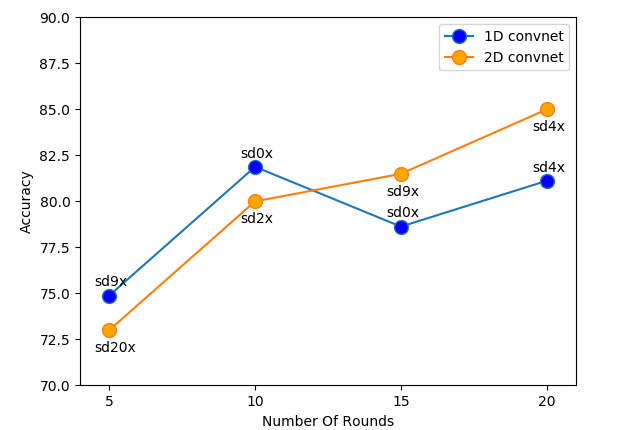
\includegraphics[width=9.8cm]{images/bestAccPlotNew.png}
		\caption[Best results for the different number of rounds before the changes to the simulator.]{Best results for the different number\\\hspace{0\textheight} of rounds before the changes to the simulator. Ratios\\\hspace{0\textheight} of real to simulated games is additionally described.}
		\label{fig:bestAccPlot}
	\end{figure}
\end{minipage}

 However, if the case, this begs the questions why this does not apply to 2D convnets. There is a possibility that the worse performance in later turns has a strong impact on the statistical features fed to the 1D convnet, but once these features are used to create the synthetic images for the 2D convnet this negative impact decreases. Figure \ref{fig:bestAccPlot} additionally shows the ratios of simulated to real data for each of the best results. The fact that the 2D convnets for 15 rounds have the best results when using 9 simulated games for each real game while the best configurations of the 1D convnets for 15 rounds use no simulations, supports the theory from above. Nonetheless the findings are not sufficient to verify the theory. For that more research would be required. However, if found to be true, it could mean that 2D convnets using synthetic images have the potential to handle inaccurate simulations better than 1D convnets. From a different perspective, this could also indicate that, assuming the simulator does actually perform worse in later rounds and is improved in that regard, the accuracy of the 1D convnets after 10 rounds could be improved.


\newpage


%beobachtung: bei 2d sind simulationen länger besser. Analysieren ob es daran liegt dass die anderen keine convergence erreichen. Wenn nicht dann ist es coole entdckung. Weil es ein anzeichen dafür ist, dass die 2d cnn besser mit simulationen lernen kann als 1d cnn. This also fits to the observation, that the results from 1dcnn with more than 10 rounds dont get much better if not worse. This can be caused by the fact that the simulations are less accurate after the first 10 steps, and therefore the 1d cnn does not improve by including them. However, the 2d cnn does improve using the last steps. This is an additional indicator, that the 2d cnn can better handle simulated games. A possibility is, that the difernce between simualted and real games in the synthetic images created using the feautre is not as siificant as when direclty using the statistical features in the 1d cnn. \todo{noch mit zahlen aus den tabelen begründen. und sagen dass die alle convergence erreichen, weshalb man das sagen kann}

% easy to believe that in some cases more the optimal ratio has not been reached yet, if only looking at the tables. However there are more factors that influnece the result. This becomes evident when plotting the trainig histories for accuracy and loss. ... plott wo wan sieht das divergence nicht erreicht wurde... The fact that the trainings with a lower ratio result in worse accuracy dont neccessarily are caused by the fact that more simulated games would be better, but could also be influenced by the fact that the divergence has not been reache yet, meaning that either a different learning rate or more epochs could increase the accuray. Therefore it can not be said with certainty that ore simulated games would in that case lead to the optimal result, as the optimal result could also be with less simulated but with changed hyper parameters. However, the hyper paramaters were intentinally chossen the same so that the results could be compared with each other.
 
It was considered to perform statistical tests comparing different models and ratios to reveal significant or insignificant differences. However, the decision was made that this does not really give reliable results, because the results are not necessarily the best achievable as the models were not individually optimized. Therefore, the results of statistical tests performed on the achieved accuracies, would not justify any statements regarding whether 1D convnets or 2D convnets perform significantly better. Such statistical tests would only show significant differences or indifferences in the results, but could not be interpreted for any valuable findings, as not all models are used to their full potential. For choosing the best configurations from those tested no statistical tests are used. Instead simply those with the highest accuracies are chosen.

%If hyper paremeters such as the leraning rate or the number of epochs are not chosen equal accross all models of one tabel (menaing all models for 1d cnns, etc) and instead would be chosen more indivuidually to optimize the models specifically for each number of rounds and ratoin between simuated and real games, the accuracie could be signifcantly different. Additionally the topologies of all models of one type are chosen the same, although this might not produce the best results for each configuration.

\begin{table}[H]
	\centering
	
	\resizebox{\columnwidth}{!}{%
		\begin{tabular}{|l||c|c|c|c|c|}
			\hline
			 & 5 r. & 10 r. & 15 r. & 20 r. & Average  \\
			\hline
			\hline
			1D convnet - before & 74.88\% (sd9x) & 81.88\% (sd0x) &78.63\% (sd0x) & 81.12\% (sd4x) & 79.13\% \\
			1D convnet - afterwards& 71.88\% (sd20x) & 81.88\% (sd0x) &78.75\% (sd5x) & 80.25\% (sd4x)  & 78.19\%  \\
			\hline
			2D convnet - before & 73.0\% (sd20x) & 80.0\% (sd2x) &81.5\% (sd9x) & 85.0\% (sd4x)  & 79.88\% \\
			2D convnet - afterwards & 71.0\% (sd6x) & 79.62\% (sd2x) & 82.25\% (sd3x) & 80.0\% (sd2x) & 78.22\% \\
			\hline
		\end{tabular}
	}
	\caption[Highest accuracies before and after the changes to the simulator.]{Highest accuracies before and after the changes to the simulator. Furthermore, the rations of simulated to real games and the average accuracies of the best results from each configuration are shown.}
	\label{tab:best_acc}
\end{table}

Table \ref{tab:best_acc} shows the best result for all categories before and after changing the simulator. It can be seen that although some accuracies are slightly better after the changes to the simulator the results are on average noticeably worse than before. The accuracy from the 2D convnet for 20 rounds, for instance, is decreased from 85.0\% to 80.0\%. The reason for this is unknown and can be highly complex, due to the many factors involved. A theory is, that reducing the randomness of the simulator and therefore making the simulated games more similar to the real games, may have resulted in a decreased generalising ability of the models and therefore less robustness on unknown data. However, this theory can hardly be verified. The overall decreased performance after the changes leads to the decision to only use the models trained on the simulated data created before the changes to the simulator. The chosen configurations for the different numbers of rounds can be seen in table \ref{tab:chosen_configs}. 

\begin{table}[H]
	\centering
	
		\begin{tabular}{|l||c|c|c|c|}
			\hline
			& 5 r. & 10 r. & 15 r. & 20 r.  \\
			\hline
			\hline
			1D convnet & 74.88\% (sd9x) & 81.88\% (sd0x) & &  \\
			\hline
			2D convnet &  & & 81.5\% (sd9x) & 85.0\% (sd4x)  \\
			\hline
		\end{tabular}
	\caption[The chosen configurations and their accuracies.]{The chosen configurations and their accuracies (averaged over 400 models each). }%\label{tab1}
	\label{tab:chosen_configs}
\end{table}

The 1D convnets trained, perform better for 5 and 10 rounds than 2D convnets, while 2D convnets perform better for 15 and 12 rounds. Depending on the number of rounds it can therefore be beneficial to use either 1D convnets or 2D convnets. The 4 best configurations for the different numbers of rounds are used in section \ref{voting} \nameref{voting}. Figures \ref{fig:1d10}, \ref{fig:1d20}, \ref{fig:2d30} and \ref{fig:2d40} show the average training and test accuracy during the course of training the models of these 4 configurations. 

\begin{minipage}{0.5\textwidth}
	\begin{figure}[H]
		\centering
		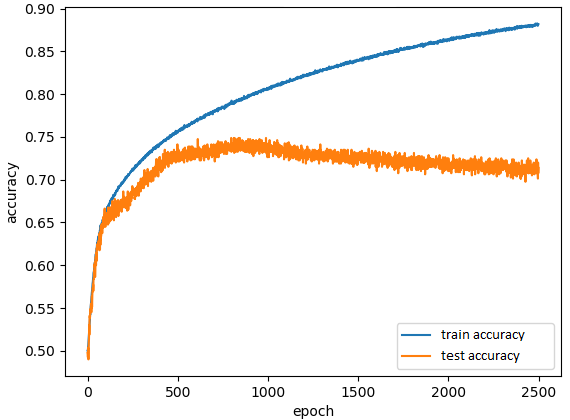
\includegraphics[width=7.5cm]{images/bestHistories/edit/1d_10s_sd9x_acc.png}
		\caption[Average training and test accuracy of 400 1D convnets on 5 rounds and a ratio of 9 simulated games for each real game.]{Average training and \\\hspace{0\textwidth}test accuracy of 400 1D convnets \\\hspace{0\textwidth}on 5 rounds and a ratio of 9 simulated  \\\hspace{0\textwidth}games for each real game. Best test \\\hspace{0\textwidth}accuracy is 74.88\% at epoch 812.}
		\label{fig:1d10}
	\end{figure}
\end{minipage}
\begin{minipage}{0.5\textwidth}
	\begin{figure}[H]
		\centering
		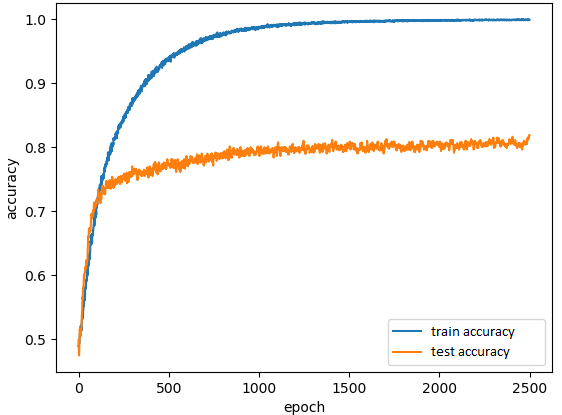
\includegraphics[width=7.5cm]{images/bestHistories/edit/1d_20s_sd0x_acc_new.png}
		\caption[Average training and test accuracy of 400 1D convnets on 10 rounds using no simulated games.]{Average training and \\\hspace{0\textwidth}test accuracy of 400 1D convnets \\\hspace{0\textwidth}on 10 rounds using no simulated \\\hspace{0\textwidth}games. Best test accuracy\\\hspace{0\textwidth} is 81.88\% at epoch 2498.}
		%\caption[Bild kurz]{Training history of 1d cnn\\\hspace{0\textwidth} on 10 rounds and using no  \\\hspace{0\textwidth} simulated games. Best validation \\\hspace{0\textwidth}accuracy is 81.12\% at epoch 1317.}
		\label{fig:1d20}
	\end{figure}
\end{minipage}

\begin{minipage}{0.5\textwidth}
	\begin{figure}[H]
		\centering
		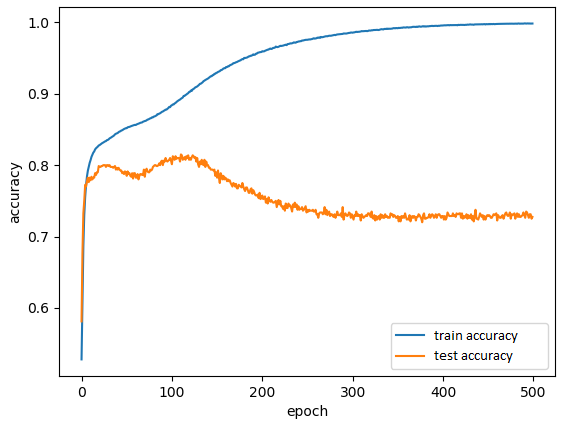
\includegraphics[width=7.5cm]{images/bestHistories/edit/2d_30s_sd9x_acc.png}
		\caption[Average training and test accuracy of 400 2D convnets on 15 rounds and a ratio of 9 simulated games for each real game.]{Average training and \\\hspace{0\textwidth}test accuracy of 400 2D convnets \\\hspace{0\textwidth}on 15 rounds and a ratio of 9 simulated  \\\hspace{0\textwidth}games for each real game. Best test \\\hspace{0\textwidth}accuracy is 81.5\% at epoch 111.}
		%\caption[Bild kurz]{Training history of 2d cnn\\\hspace{0\textwidth} on 10 rounds and a ratio of 9 simulated  \\\hspace{0\textwidth}games for each real game. Best validation \\\hspace{0\textwidth}accuracy is 74.88\% at epoch 812.}
		%\caption[Bild kurz]{best validation \\\hspace{0\textwidth}accuracy 81.5\% (at epoch 111)}
		\label{fig:2d30}
	\end{figure}
\end{minipage}
\begin{minipage}{0.5\textwidth}
	\begin{figure}[H]
		\centering
		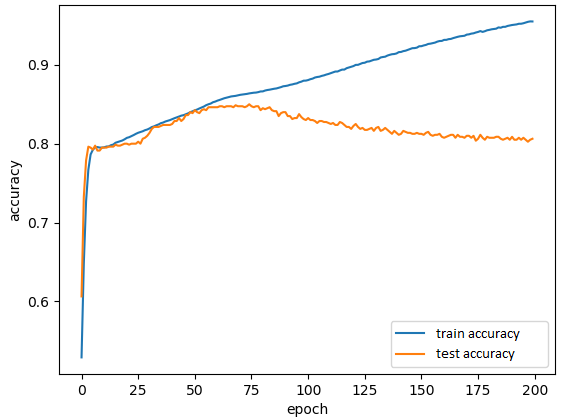
\includegraphics[width=7.5cm]{images/bestHistories/edit/2d_40s_sd4x_acc.png}
		\caption[Average training and test accuracy of 400 2D convnets on 20 rounds and a ratio of 4 simulated games for each real game.]{Average training and \\\hspace{0\textwidth}test accuracy of 400 2D convnets \\\hspace{0\textwidth}on 20 rounds and a ratio of 4 simulated \\\hspace{0\textwidth}games for each real game. Best test \\\hspace{0\textwidth}accuracy is 85.0\% at epoch 75.}
		%\caption[Bild kurz]{Training history of 1d cnn\\\hspace{0\textwidth} on 10 rounds and a ratio of 9 simulated  \\\hspace{0\textwidth}games for each real game. Best validation \\\hspace{0\textwidth}accuracy is 74.88\% at epoch 812.}
		%\caption[Bild kurz]{best validation \\\hspace{0\textwidth}accuracy 85.0\% (at epoch 75)}
		\label{fig:2d40}
	\end{figure}
\end{minipage}

%Due to complications many configurations had to be retrained. As it was known from prior tests that certain configurations do not improve after a certain number of epochs and due to the time constraints of this work the models were retrained with not as many epochs to save time. For instant the test accuracies of the 2D convnets trained on 20 rounds do not improve any more after around 60 or 70 epochs and therefore the retraining of the models was only done on 200 epochs as shown in figure \ref{fig:2d40}. 

%- vielleiht gucken welche falsch erkannt werden und woran es liegt, also wenn die zum beispiel echt schlect oder gut sind obwohl es nicht so sein sollte (rausnhemen und gucken wie ergebnisse sind, vielleicht nur bei bestem modell) -> glaube eher nicht\\
%- training auf welchem rechner/n,was von: cpu oder gpu oder beides, hardware kurz erwähnen, vpn (fernzugriff)\\
%- train test splt, leave one out k fold (+ begründung mit deep learing ..reliable results etc, randomness) \\
%- kurz erklären wieso weniger züge besser sind bei dieser hci erkennung\\
%- (vielleicht kram zu adaptive learning rate ändern und gucken wie es so ist, ansonsten begründen wieso ich das nicht brauche) \\
%- (entweder so dass 1d cnn mit 20 steps auch konvergence erreicht oder danach nochmal anpassung von 20 steps 1d cnn damit es kovergiert)\\
%- darüber schreiben dass letzen n züge nicht mehr so gut simuliert sind (zeigen) und deshalb 40 steps nicht so viel besser ist (glaube nicht dass es so ist, also wahrscheinlich auslassen. Vielleicht bei 15r 1dnn aber man kann es schwer relaible begründen)\\
%- mit maximalen guten steps (glaube 16 züge oder so) trainieren und vergleichen\\
%- statistical tests um signifikante unterschiede /keine unterschiede zu zeigen für verschiedene modelle etc (siehe mazens nachricht) ? \\
